% Informe del Proyecto Final de EDA 2026-2.
% Compilar desde report/:  latexmk -pdf informe.tex
% (o: python scripts/build_report.py --group Grupo2, que además renombra el PDF)
\documentclass[11pt,letterpaper]{article}

\usepackage[T1]{fontenc}
\usepackage[utf8]{inputenc}
\usepackage{lmodern}
\usepackage{textcomp}
\usepackage{amsmath,amssymb}
\usepackage[spanish,es-noshorthands,es-tabla,es-nodecimaldot]{babel}
\usepackage{newunicodechar}
\newunicodechar{µ}{\textmu}
\usepackage[top=2.3cm,bottom=2.3cm,left=2.3cm,right=2.3cm,headheight=14pt]{geometry}
\usepackage{graphicx}
\usepackage{booktabs}
\usepackage{tabularx}
\usepackage{array}
\usepackage{float}
\usepackage[font=small,labelfont=bf,skip=4pt]{caption}
\usepackage{enumitem}
\usepackage{fancyhdr}
\usepackage{titlesec}
\usepackage{xcolor}
\usepackage{fancyvrb}
\usepackage{microtype}
\usepackage[hidelinks]{hyperref}
\hypersetup{colorlinks=true,linkcolor=black,citecolor=black,urlcolor=blue!60!black,
  pdftitle={Proyecto Final EDA 2026-2: pipeline de data streams para comercio electrónico},
  pdfauthor={Garcia Villacorta, Barreto Daza, Chulluncuy Reynoso, Hilario Orihuela}}

\newcommand{\repo}{https://github.com/dantebarreto-gif/Proyecto-Final-E-AD}
\newcommand{\Oh}[1]{\ensuremath{O(#1)}}

\setlist[itemize]{label=\scriptsize$\blacksquare$,itemsep=2pt,topsep=4pt}
\setlist[enumerate]{itemsep=2pt,topsep=4pt}
\setlength{\parskip}{4pt}
\renewcommand{\topfraction}{0.9}
\renewcommand{\bottomfraction}{0.8}
\renewcommand{\textfraction}{0.07}
\renewcommand{\floatpagefraction}{0.8}
\setlength{\parindent}{0pt}
\renewcommand{\arraystretch}{1.15}
\newcolumntype{L}{>{\raggedright\arraybackslash}X}

\pagestyle{fancy}
\fancyhf{}
\fancyhead[L]{Pipeline de Data Streams --- Proyecto Final}
\fancyhead[R]{\thepage}
\renewcommand{\headrulewidth}{0.6pt}

\titleformat{\section}{\Large\bfseries}{\thesection.}{0.6em}{}
\titleformat{\subsection}{\large\bfseries}{\thesubsection.}{0.6em}{}
\titlespacing*{\section}{0pt}{14pt}{6pt}
\titlespacing*{\subsection}{0pt}{10pt}{4pt}

\begin{document}

% ---------------- Portada ----------------
\begin{titlepage}
  \centering
  \vspace*{0.4cm}
  
\includegraphics[width=5cm]{img/utec_posgrado.png}\par
  \vspace{0.9cm}
  {\LARGE\bfseries UNIVERSIDAD DE INGENIERÍA Y TECNOLOGÍA\par}
  \vspace{2pt}
  {\large\bfseries ESCUELA DE POSGRADO\par}
  \vspace{1.1cm}
  \rule{\textwidth}{0.6pt}\par\vspace{0.5cm}
  {\large\bfseries Proyecto Final: Estructuras de Datos Avanzadas Orquestadas\par}
  \vspace{4pt}
  {\bfseries Pipeline eficiente de procesamiento de data streams para comercio electrónico (Escenario B)\par}
  \vspace{0.4cm}\rule{\textwidth}{1.2pt}\par
  \vspace{1.4cm}
  {\bfseries AUTOR(ES)\par}\vspace{6pt}
  Sebastian Rodrigo Garcia Villacorta\\
  Dante Guillermo Barreto Daza\\
  Clinton Michael Chulluncuy Reynoso\\
  Ronald Ramiro Hilario Orihuela\par
  \vspace{0.45cm}
  {\bfseries DOCENTE\par}\vspace{6pt}
  Heider Sánchez\par
  \vspace{0.45cm}
  {\bfseries CURSO\par}\vspace{6pt}
  Estructuras de Datos y Algoritmos\par
  \vspace{0.45cm}
  {\bfseries REPOSITORIO\par}\vspace{6pt}
  \url{\repo}\par
  \vfill
  Lima -- Perú\par
  \vspace{4pt}
  2026\par
\end{titlepage}

\tableofcontents
\newpage

% ---------------- Resumen ----------------
\section*{Resumen}
\addcontentsline{toc}{section}{Resumen}

Se construyó un pipeline de 10 etapas que procesa de punta a punta \textbf{10\,223\,169 eventos reales} del dataset REES46 (los primeros 10M de octubre de 2019, más el componente de stream sintético que pide el enunciado) a 8\,204 eventos por segundo en Python, con todas las estructuras implementadas desde cero: cola FIFO enlazada, merge sort y búsqueda binaria, heap binario, tabla hash, caché LRU, matriz dispersa, B+Tree en disco, KD-Tree, Bloom Filter, Count-Min Sketch, MinHash + LSH, IVF y HNSW, PageRank, Louvain, Label Propagation y Trie. El filtro de fraude bloquea 70\,682 eventos con precisión de 92{,}9\,\% y recall de 91{,}1\,\% usando 3{,}4\,KB para la lista negra, y sus falsos positivos son cuentas reales con ráfagas de hasta 110 carritos o compras en 10 minutos. El B+Tree responde una búsqueda sobre 10M claves en 44\,µs con altura 3; el KD-Tree resuelve KNN 537 veces más rápido que fuerza bruta; LSH responde consultas de similitud 295 veces más rápido que la comparación exhaustiva con recall@10 de 1{,}0 sobre los vecinos relevantes. Los experimentos de 1K a 10M confirman en escala log-log las complejidades teóricas, y un mismo evento queda trazado a través de las 10 etapas.

\textbf{Repositorio:} \url{\repo}\\
Contiene el código fuente, este informe (fuente \LaTeX{} en \texttt{report/informe.tex}), el notebook de análisis, el diagrama del pipeline, los CSV de los experimentos, las diapositivas y la tabla de roles del equipo.

% ---------------- 1 ----------------
\section{Contexto y objetivo}

Una tienda en línea recibe un flujo continuo de vistas, carritos y compras. Sobre ese flujo hay que priorizar órdenes urgentes, consultar productos con baja latencia, detectar fraude en segundos, recomendar productos relacionados y descubrir qué productos se compran juntos. Cada problema tiene una estructura de datos adecuada; el objetivo del proyecto es encadenarlas de modo que la salida de cada etapa sea la entrada real de la siguiente, y medir cuánto ganan las estructuras aproximadas frente a sus alternativas exactas.

\textbf{Datos.} Se usa el dataset REES46 \emph{eCommerce behavior data from multi category store} (Kaggle, \texttt{mkechinov/ecommerce-behavior-data-from-multi-category-store}; archivos de octubre y noviembre de 2019 con 110M eventos y columnas \texttt{event\_time}, \texttt{event\_type}, \texttt{product\_id}, \texttt{category\_id}, \texttt{category\_code}, \texttt{brand}, \texttt{price}, \texttt{user\_id}, \texttt{user\_session}). DuckDB lee \texttt{2019-Oct.csv} (5{,}7\,GB) en streaming y toma los \textbf{primeros 10M eventos en orden temporal}, del 1 al 8 de octubre de 2019: 120\,565 productos, 1\,072\,341 usuarios y un embudo muy desbalanceado (95{,}6\,\% vistas, 2{,}2\,\% carritos y 2{,}2\,\% compras). El catálogo se deriva de los mismos eventos y las filas sin sesión se agrupan por usuario. Como pide el enunciado, el componente de stream es sintético y se agrega con semilla fija: identificador de evento, dispositivo, IP, tarjeta, usuario premium, tipo de envío (express, estándar, programado), consultas de búsqueda, \textbf{1{,}5\,\% de duplicados} reenviados segundos después y \textbf{ráfagas de fraude} (25 a 120 intentos en menos de 5 minutos desde una tarjeta y un dispositivo). La mitad de las tarjetas fraudulentas se asume ya reportada (lista negra). El repositorio incluye además un generador con el mismo esquema, que se usa en las pruebas y en los experimentos de escalabilidad, donde el tamaño de la entrada debe controlarse.

% ---------------- 2 ----------------
\section{Arquitectura del pipeline}

\begin{figure}[!htbp]
  \centering
  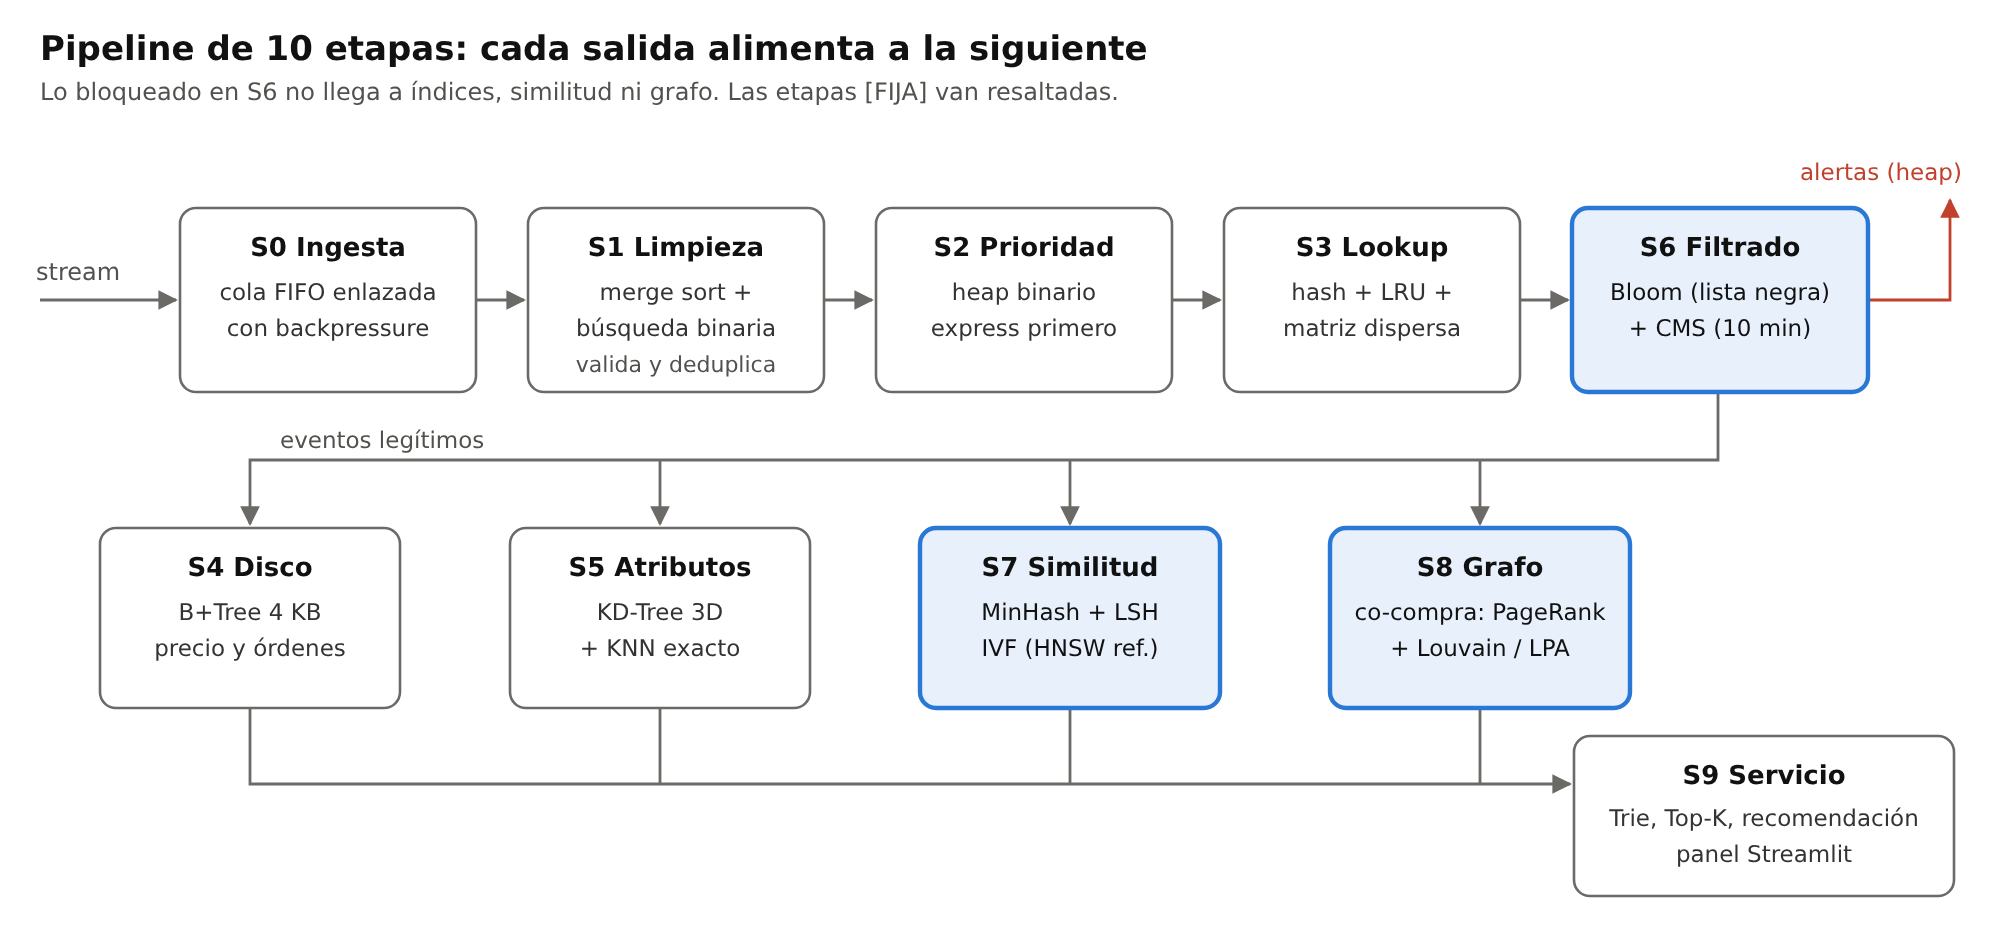
\includegraphics[width=\linewidth]{../docs/pipeline.png}
  \caption{Flujo por lote. S6 se ejecuta inmediatamente después de S3: solo lo que pasa el filtro llega a S4, S5, S7 y S8, y todas las salidas convergen en S9.}
  \label{fig:pipeline}
\end{figure}

El stream se procesa en lotes de 5\,000 eventos. Las etapas incrementales (S0 a S4, S6, S8 y S9) actúan sobre cada evento; las estructuras estáticas o costosas de construir (KD-Tree, firmas MinHash, SVD + IVF, PageRank y Louvain) se \textbf{refrescan} cada 2M eventos y al final, como en un sistema lambda con capa rápida y capa por lotes. Cada etapa deja una nota en la traza del evento, lo que permite verificar la integración de forma observable (sección~\ref{sec:integracion}).

% ---------------- 3 ----------------
\section{Etapas 0 a 5: estructuras base}

\begin{table}[!htbp]
\centering\footnotesize
\begin{tabularx}{\linewidth}{@{}p{1.9cm}LLp{2.7cm}p{2.5cm}@{}}
\toprule
\textbf{Etapa} & \textbf{Estructura} & \textbf{Función en el pipeline} & \textbf{Complejidad} & \textbf{Alternativa descartada}\\
\midrule
0 Ingesta & Cola FIFO con lista enlazada y capacidad máxima & Buffer entre el lector y el consumidor por lotes; descarta y cuenta si se llena (backpressure) & enqueue/dequeue $O(1)$ & Lista de Python: \texttt{pop(0)} es $O(n)$\\
1 Preprocesa\-miento & Merge sort estable + búsqueda binaria vectorizada & Valida y normaliza; busca cada id en la ventana ordenada de los últimos 500K ids y elimina duplicados; reordena por tiempo & $O(b\log b)$ por lote; $O(b\log W)$ contra la ventana & Conjunto de todos los ids: memoria sin límite\\
2 Prioridad & Heap binario (min-heap) con desempate por llegada & Compras express, premium, estándar, programadas, carritos y vistas; ordena también las alertas de fraude & push/pop $O(\log n)$, heapify $O(n)$ & Lista ordenada: inserción $O(n)$\\
3 Almacena\-miento & Tabla hash (sondeo lineal, carga $\le 0{,}7$, lápidas), caché LRU, matriz dispersa DOK $\to$ CSR & Resuelve \texttt{product\_id} y \texttt{user\_id} a índices densos; cachea fichas y recomendaciones; matriz usuario $\times$ producto (vista 1, carrito 3, compra 5) & $O(1)$ amortizado; CSR con nnz valores & Matriz densa: $200\text{K}\times200\text{K}$ no cabe\\
4 Índice en disco & B+Tree con páginas de 4\,KB (255 claves por hoja), hojas encadenadas, buffer pool LRU con write-back & Índice de precio (carga masiva) e índice temporal de órdenes legítimas (inserciones); consultas por rango & búsqueda $O(\log_B n)$ páginas; rango $O(\log_B n + k/B)$ & Árbol binario: altura $\log_2 n$, una página por nodo\\
5 Multidi\-mensional & KD-Tree (corte por mediana en el eje más extendido, hojas de 16) y KNN exacto & Vecinos por log precio, log vistas y tasa de conversión; consultas por caja & construcción $O(n\log n)$; KNN $\approx O(\log n)$ en $d$ bajo & Fuerza bruta $O(n)$ por consulta\\
\bottomrule
\end{tabularx}
\caption{Estructuras base, su función y su complejidad.}
\end{table}

La clave del índice de precio combina precio en centavos e índice de producto (\texttt{precio·100 << 24 | id}), única y ordenada por precio. Con 10M claves el B+Tree tiene altura 3, así que una búsqueda lee como máximo 3 páginas.

% ---------------- 4 ----------------
\section{Bloque de investigación avanzada (etapas 6 a 8)}

\subsection{Filtrado probabilístico: Bloom Filter y Count-Min Sketch}

\textbf{Bloom Filter} (Bloom, 1970). Arreglo de $m$ bits y $k$ funciones hash: insertar pone $k$ bits en 1; consultar responde ``posiblemente presente'' si los $k$ están en 1. No hay falsos negativos y la tasa de falsos positivos es
\[ p \approx \left(1 - e^{-kn/m}\right)^{k}, \qquad m = -\frac{n \ln p}{(\ln 2)^2}, \qquad k = \frac{m}{n}\ln 2, \]
de modo que para $p = 1$\,\% bastan 9{,}6 bits por elemento y $k = 7$, sin importar el tamaño de la clave. Las $k$ posiciones se obtienen con doble hashing $g_i = h_1 + i\,h_2 \bmod m$ (Kirsch y Mitzenmacher, 2006) sobre splitmix64, y los bits van empaquetados en un arreglo \texttt{uint8}; cada operación cuesta $O(k)$. \textbf{Uso:} lista negra de tarjetas y dispositivos. Como un positivo puede ser falso y bloquear una compra es una decisión crítica, todo positivo se verifica contra el conjunto exacto antes de bloquear. \textbf{Límite:} no admite borrado (sí con contadores, Counting Bloom) y la tasa de falsos positivos crece si se supera la capacidad.

\textbf{Count-Min Sketch} (Cormode y Muthukrishnan, 2005). Matriz de $d \times w$ contadores con un hash por fila; la estimación es el mínimo de las $d$ celdas. Nunca subestima y, con $w = \lceil e/\varepsilon \rceil$ y $d = \lceil \ln(1/\delta) \rceil$, cumple $\hat f \le f + \varepsilon N$ con probabilidad $1-\delta$. La memoria $O(w\,d)$ no depende del número de claves. \textbf{Uso:} clave = tarjeta y, por separado, dispositivo; \textbf{ventana} de 10 minutos en un anillo de 10 sub-sketches de 1 minuto (al avanzar se limpia el más viejo); \textbf{umbral} de más de 12 intentos de compra o carrito por tarjeta, o 20 por dispositivo, dentro de la ventana. La sobreestimación solo puede adelantar una alerta, nunca ocultarla.

\subsection{Similitud de conjuntos: MinHash + LSH}

Para una permutación aleatoria $h$, $P[\min h(A) = \min h(B)] = J(A,B)$ (Broder, 1997): la fracción de coincidencias entre dos firmas de $P$ minhashes estima Jaccard con error estándar $\sqrt{J(1-J)/P}$. Con LSH por bandas (Indyk y Motwani, 1998) la firma se corta en $b$ bandas de $r$ filas, y dos conjuntos son candidatos si coinciden en una banda completa:
\[ P[\text{candidato}] = 1 - \left(1 - J^{r}\right)^{b}, \qquad \text{umbral} \approx (1/b)^{1/r}. \]
Se eligió MinHash (y no SimHash) porque el objeto natural es un \textbf{conjunto}: los usuarios que pusieron cada producto en el carrito o lo compraron. Con $P = 128$, $b = 32$ y $r = 4$ el umbral es 0{,}42. Las 32 bandas se indexan en \textbf{un solo arreglo ordenado} de pares (hash de banda mezclado con el número de banda, id), y una consulta son dos búsquedas binarias vectorizadas, la misma estructura de la etapa 1. Construcción $O(P \cdot \mathrm{nnz})$; consulta $O(b \log(nb) + \text{candidatos})$.

\subsection{ANN vectorial: IVF (y HNSW como referencia)}

Los productos se representan con embeddings de 32 dimensiones obtenidos por \textbf{SVD truncada aleatorizada} (Halko et al., 2011) de la matriz usuario $\times$ producto en CSR, implementada solo con productos matriz-vector. \textbf{IVF} (índice de archivo invertido; Jégou et al., 2011): k-means (k-means++ y Lloyd) divide el espacio en $n_\text{list} = 4\sqrt{n}$ celdas (máximo 4096); cada vector se guarda en la lista de su centroide y una consulta recorre solo las $n_\text{probe}$ listas más cercanas, con costo $O(n_\text{list}\,d + n_\text{probe}\,(n/n_\text{list})\,d)$. \textbf{HNSW} (Malkov y Yashunin, 2020): grafo navegable en capas con nivel geométrico por nodo, descenso greedy en las capas altas y búsqueda best-first con $ef$ candidatos en la capa 0, con la heurística de vecinos diversos del artículo; $O(\log n)$ esperado. Se eligió IVF para el pipeline porque su construcción y consulta son operaciones de matriz (escala a 10M en Python), y HNSW se implementó para comparar el compromiso recall/latencia. La línea base es KNN exacto por fuerza bruta, $O(n\,d)$; el KD-Tree de la etapa 5 sirve de contraste, porque en $d = 32$ deja de podar.

\subsection{Ranking de influencia: PageRank}

El grafo de co-compra es no dirigido y ponderado: nodos = productos y $w(u,v)$ = número de órdenes (compras de una misma sesión) que contienen a ambos. PageRank (Brin y Page, 1998) es el vector estacionario de una caminata aleatoria que sigue aristas con probabilidad proporcional al peso y salta a un nodo aleatorio con probabilidad $1-\alpha$ ($\alpha = 0{,}85$):
\[ r \leftarrow \alpha\left(P^{\top} r + \text{masa colgante}\cdot v\right) + (1-\alpha)\,v. \]
Se implementa con iteración de potencias sobre la CSR ($O(m)$ por iteración, hasta que la norma $L_1$ del cambio sea menor que $10^{-9}$) y se valida contra NetworkX. La versión personalizada ($v$ concentrado en los productos del usuario) da recomendaciones locales. La línea base es el grado ponderado; PageRank, en cambio, premia estar conectado con productos a su vez centrales, no solo tener muchas co-compras.

\subsection{Comunidades: Louvain frente a Label Propagation}

\textbf{Louvain} (Blondel et al., 2008) maximiza la modularidad
\[ Q = \sum_{c}\left[\frac{L_c}{2m} - \left(\frac{d_c}{2m}\right)^{2}\right] \]
en dos fases repetidas: mover cada nodo a la comunidad vecina con mayor ganancia $\Delta Q \propto k_{i,c} - \Sigma_\text{tot}\,k_i/2m$, y luego colapsar cada comunidad en un nodo; casi $O(m \log n)$. \textbf{Label Propagation} (Raghavan et al., 2007): cada nodo adopta la etiqueta de mayor peso entre sus vecinos hasta que no hay cambios; es casi lineal pero no optimiza una función objetivo, por lo que es menos estable. La estabilidad se mide con la información mutua normalizada (NMI) entre corridas con distinta semilla. Leiden (Traag et al., 2019) corrige comunidades mal conectadas de Louvain y queda como trabajo futuro.

% ---------------- 5 ----------------
\section{Diseño de la integración}\label{sec:integracion}

La integración se verifica con un evento concreto. En la corrida de 10M se trazó automáticamente una compra legítima ubicada al 70\,\% del stream; la Figura~\ref{fig:traza} muestra su salida literal.

\begin{figure}[!htbp]
\begin{Verbatim}[fontsize=\footnotesize,frame=single,framesep=6pt,rulecolor=\color{black!30}]
Event(id=6966919, purchase, product=1004856, user=528344847, price=131.76)
  [S0] encolado (cola=1413)
  [S1] válido, normalizado y no duplicado
  [S2] prioridad 3 (compra programada), posición 133 de 4929 en el lote
  [S3] producto #861 y usuario #746718 resueltos en la tabla hash
  [S6] pasa el filtro (Bloom: ausente; CMS bajo el umbral)
  [S4] orden indexada por tiempo en el B+Tree
  [S5] vecinos por atributos (KD-Tree): [786, 840, 14608]
  [S7] relacionados LSH: []; vecinos IVF: [87190, 87862, 40728]
  [S8] primera compra de la orden: nodo listo para nuevas aristas
  [S9] recomendaciones Top-5 para su producto:
       samsung smartphone 4767   puntaje=1.689  fuentes=grafo+KD-Tree
       samsung smartphone 4833   puntaje=1.448  fuentes=grafo+KD-Tree
       samsung smartphone 4750   puntaje=1.024  fuentes=grafo
       generic unknown 8289      puntaje=1.001  fuentes=IVF
       samsung smartphone 4836   puntaje=0.954  fuentes=grafo
\end{Verbatim}
\caption{Recorrido de un evento por las 10 etapas en la corrida de 10M (salida de \texttt{scripts/run\_pipeline.py}).}
\label{fig:traza}
\end{figure}

Es la compra de un Samsung de 131{,}76 USD, el producto con mayor PageRank del grafo. Tiene envío programado, así que el heap la deja en la posición 133 de 4\,929, detrás de las compras express, premium y estándar del lote. LSH no devolvió candidatos porque ningún producto supera el umbral de Jaccard ($\approx 0{,}42$) con su conjunto de compradores; la recomendación final combina el grafo de co-compra, el KD-Tree (smartphones de la misma marca y rango de precio) y el IVF, y la fuente de cada producto queda registrada.

Cada flecha de la Figura~\ref{fig:pipeline} corresponde a un dato que la etapa siguiente consume: los índices densos de S3 son las filas y columnas de la matriz dispersa y los nodos del grafo; la matriz alimenta las firmas MinHash y la SVD de S7; las aristas de co-compra de S8 y su PageRank ponderan el ranking final de S9, que además usa los vecinos del KD-Tree (S5) y cachea el resultado en el LRU (S3). Las alertas de S6 se ordenan en un heap por severidad (lista negra antes que frecuencia) y las etiquetas de verdad (\texttt{is\_fraud}, \texttt{is\_duplicate}) se usan solo para medir, nunca para decidir. Hay 19 pruebas automáticas: cada estructura contra su versión exacta (\texttt{dict}, \texttt{set}, \texttt{numpy.searchsorted}, NetworkX para PageRank, fuerza bruta para KNN y Jaccard) y una prueba de integración que exige que el evento trazado pase por las etapas en el orden esperado.

% ---------------- 6 ----------------
\section{Resultados experimentales}

\textbf{Metodología.} Tamaños de 1K a 10M; 100 repeticiones para 1K y 10K, 10 para 100K, 3 para 1M y 1 para 10M (con 100 repeticiones, la serie de 10M habría tomado días en Python puro). Se reporta la media y la desviación estándar (banda sombreada en las figuras), el pico de memoria con \texttt{tracemalloc} y la pendiente en log-log como exponente empírico. Semilla fija 2026; máquina de 4 vCPU y 16\,GB, Python 3.13 y NumPy 2.5 (\texttt{results/bench/platform.json}). Todos los CSV están en \texttt{results/bench/}. Estos experimentos usan entradas generadas (claves, conjuntos, vectores y grafos con estructura conocida) para controlar $n$ y tener la respuesta exacta; la corrida del pipeline (sección~\ref{sec:corrida}) usa los datos reales.

\subsection{Estructuras base}

\begin{figure}[!htbp]
  \centering
  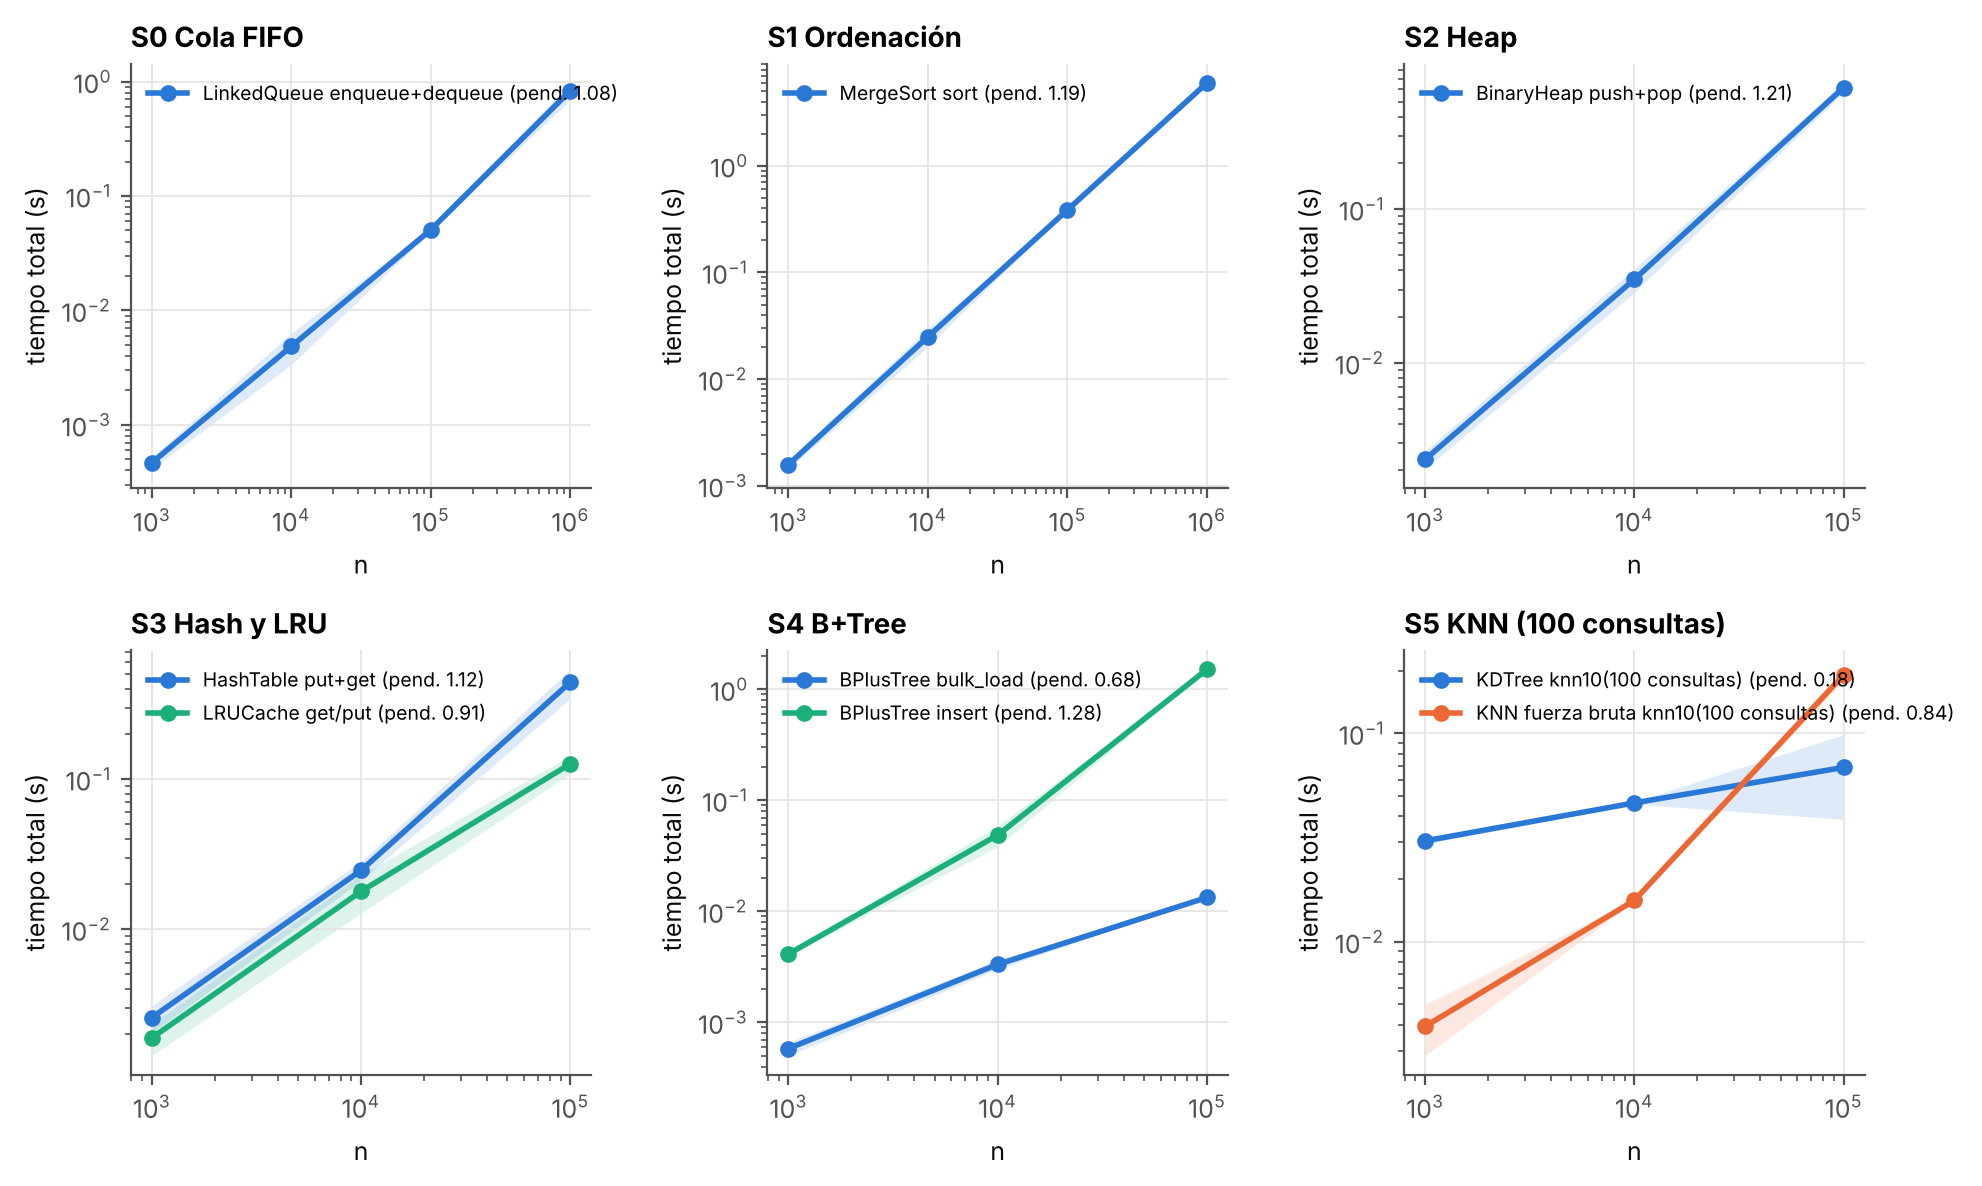
\includegraphics[width=\linewidth]{figures/fig_base_scaling.png}
  \caption{Tiempo total frente a $n$ (log-log), de 1K a 10M operaciones. La pendiente ajustada aparece en la leyenda.}
\end{figure}

\begin{table}[!htbp]
\centering\small
\begin{tabularx}{\linewidth}{@{}p{3.4cm}p{2.0cm}p{1.4cm}p{1.9cm}L@{}}
\toprule
\textbf{Estructura ($n$ = 10M)} & \textbf{Tiempo total} & \textbf{Por op.} & \textbf{Pendiente} & \textbf{Observación}\\
\midrule
Cola FIFO (enqueue + dequeue) & 13{,}7 s & 0{,}69 µs & 1{,}12 & Lineal, como se espera de $O(1)$ por operación\\
Merge sort & 111 s & 11{,}1 µs & 1{,}21 & El factor $\log n$ eleva la pendiente sobre 1\\
Heap binario (push + pop) & 181 s & 9{,}1 µs & 1{,}22 & Igual: $O(n\log n)$ en total\\
Tabla hash (put + get) & 47{,}9 s & 2{,}4 µs & 1{,}08 & 2{,}11 sondeos por operación con carga $\le 0{,}7$; 402\,MB de pico\\
Caché LRU & 11{,}2 s & 1{,}1 µs & 0{,}94 & 91{,}5\,\% de aciertos con accesos Zipf\\
B+Tree: carga masiva / búsqueda & 2{,}0 s / 44 µs & & 0{,}89/0{,}32 & Altura 3, 43\,862 páginas, 171\,MB en disco\\
KD-Tree: KNN ($k = 10$) & 0{,}73 ms por consulta & & 0{,}11 & \textbf{537 veces} más rápido que fuerza bruta (393 ms)\\
\bottomrule
\end{tabularx}
\caption{Estructuras base con $n$ = 10M.}
\end{table}

La búsqueda en el B+Tree crece de 26\,µs a 44\,µs entre 1M y 10M porque la altura pasa de 2 a 3 páginas. La inserción una a una (44\,µs, pendiente 1{,}36) se midió hasta 1M y se omitió en 10M por tiempo, unos 7 minutos adicionales sin información nueva, porque el pipeline usa carga masiva para el índice de precio.

\subsection{Filtrado probabilístico (S6)}

\begin{figure}[!htbp]
  \centering
  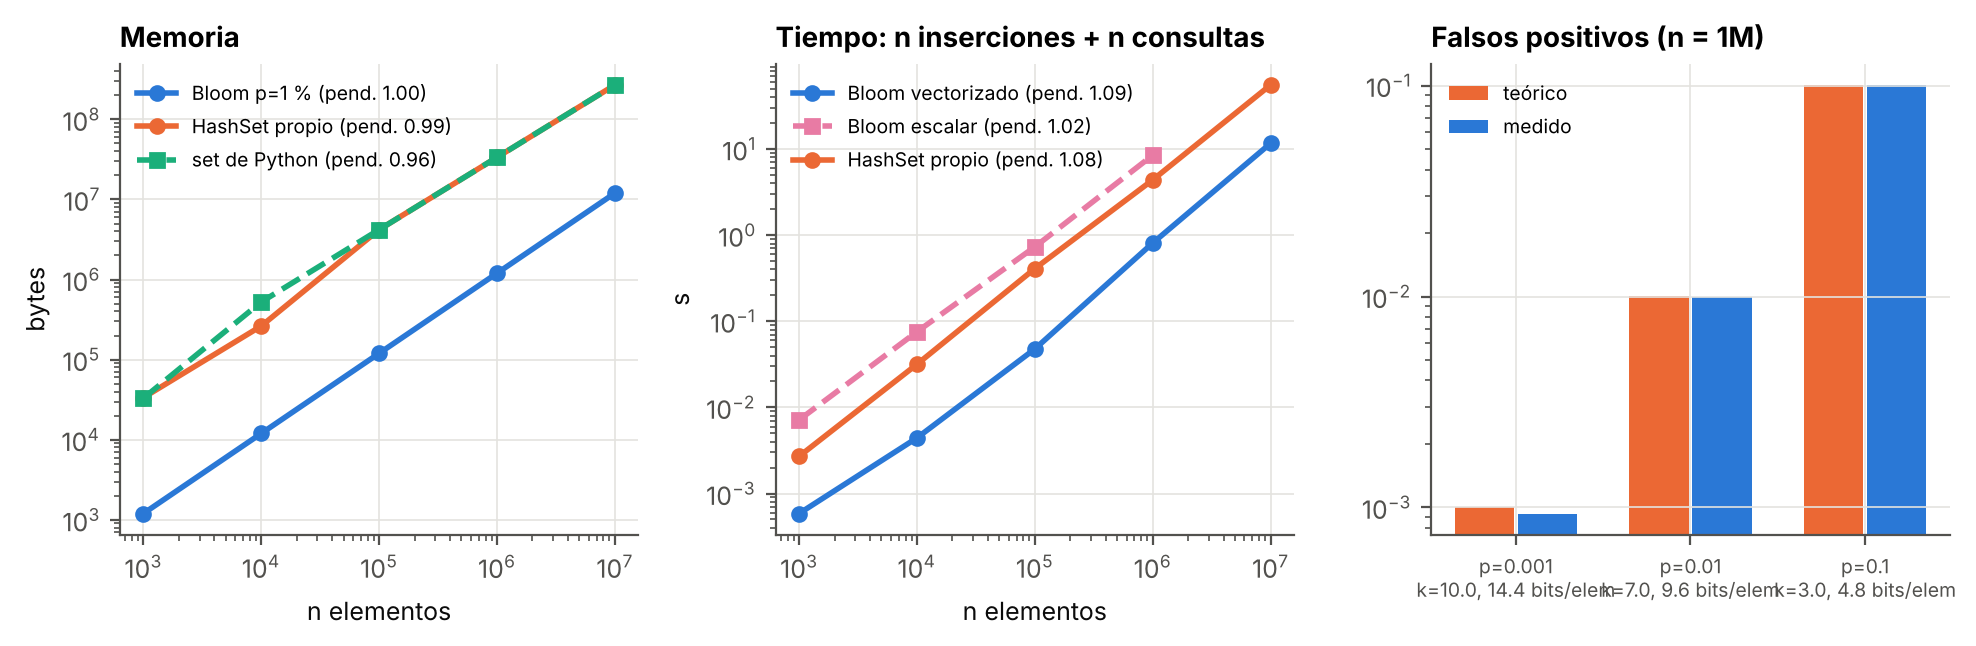
\includegraphics[width=\linewidth]{figures/fig_bloom.png}
  \caption{Bloom Filter frente a la tabla hash exacta propia y al \texttt{set} de Python: memoria, tiempo y tasa de falsos positivos teórica frente a medida.}
\end{figure}

Con 10M elementos el Bloom ($p = 1$\,\%) ocupa \textbf{12\,MB frente a 268\,MB} de la tabla exacta (22 veces menos) y es 4{,}8 veces más rápido en inserción y consulta. La tasa medida de falsos positivos coincide con la teórica en los tres valores de $p$ (0{,}0935\,\% frente a 0{,}1000\,\% con $p = 0{,}1$\,\%; 0{,}99\,\% frente a 1{,}00\,\% con $p = 1$\,\%), y nunca hubo falsos negativos. La versión vectorizada con NumPy es 10 veces más rápida que la escalar con el mismo algoritmo.

\begin{figure}[!htbp]
  \centering
  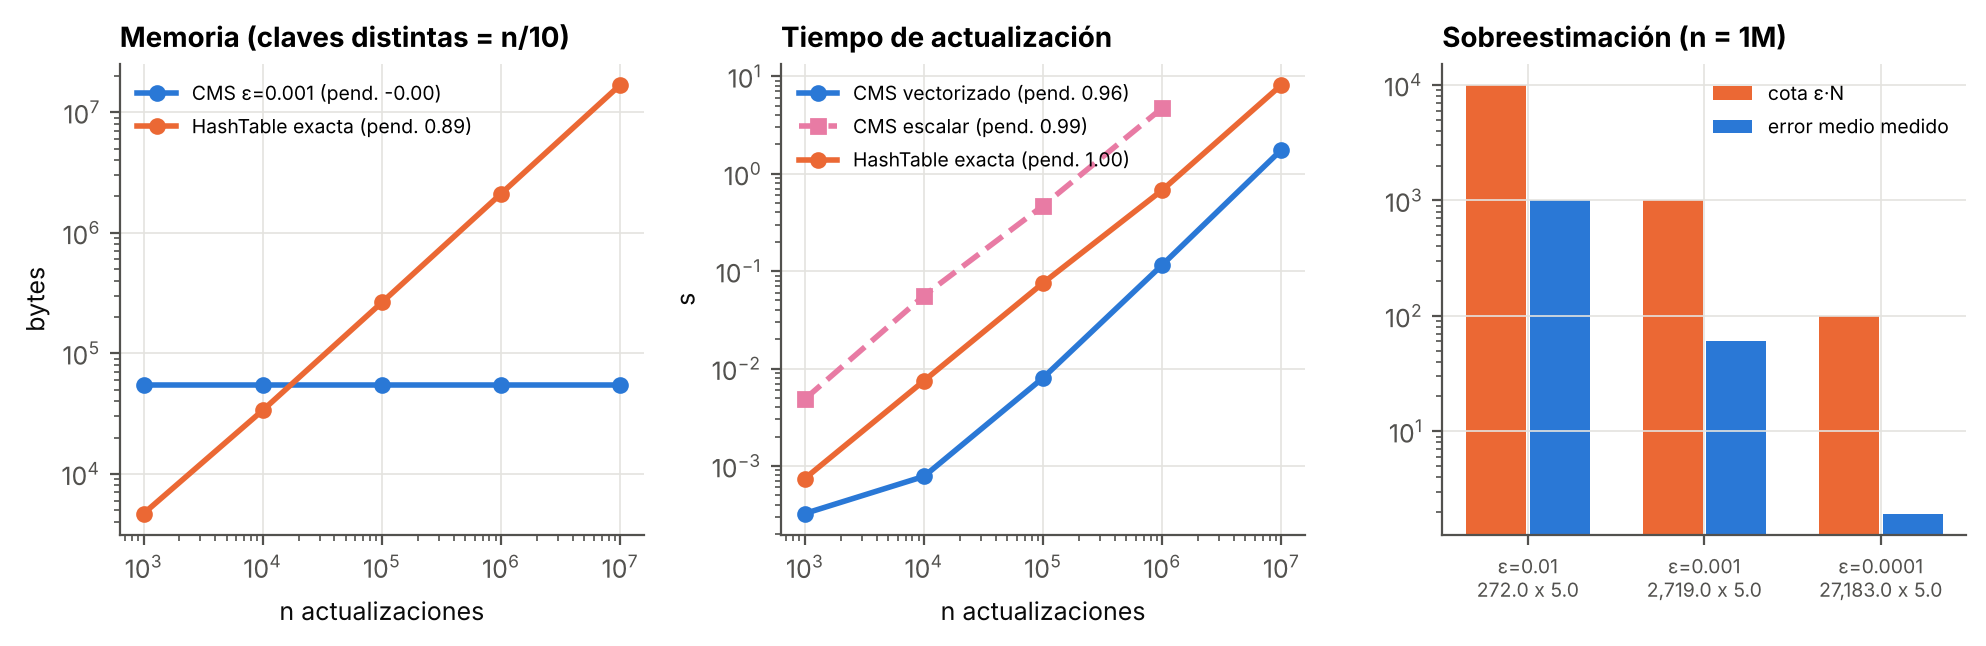
\includegraphics[width=\linewidth]{figures/fig_cms.png}
  \caption{Count-Min Sketch frente a la tabla hash exacta: memoria, tiempo de actualización y error frente a la cota $\varepsilon N$.}
\end{figure}

Con 10M actualizaciones sobre 1M claves, el CMS con $\varepsilon = 0{,}001$ usa \textbf{53\,KB frente a 16{,}8\,MB} y actualiza 4{,}6 veces más rápido. El error medio (642) y el máximo (4\,146) quedan bajo la cota $\varepsilon N = 9\,997$ en el 100\,\% de las claves, sin subestimar nunca; para las claves frecuentes, que son las que disparan alertas, el error relativo es 4\,\%. En el pipeline con los 10M eventos reales el filtro bloquea 70\,682 eventos con precisión de \textbf{92{,}9\,\%} y recall de \textbf{91{,}1\,\%}; los 7 falsos positivos del Bloom se descartaron en la verificación exacta. El recall no llega a 100\,\% porque los primeros intentos de cada ráfaga pasan antes de superar el umbral. Los falsos positivos (unos 5\,000 eventos) no son errores del sketch: en los datos reales hay 309 usuarios con más de 12 carritos o compras en una ventana de 10 minutos, hasta 110, un patrón de bot o revendedor que la etiqueta sintética no marca como fraude. Con datos sintéticos, donde ese comportamiento no existe, la precisión fue de 99{,}998\,\% (\texttt{results/demo/summary\_10M\_sintetico.json}). En producción esas alertas irían a revisión manual en lugar de bloquearse.

\subsection{Similitud (S7)}

\begin{figure}[!htbp]
  \centering
  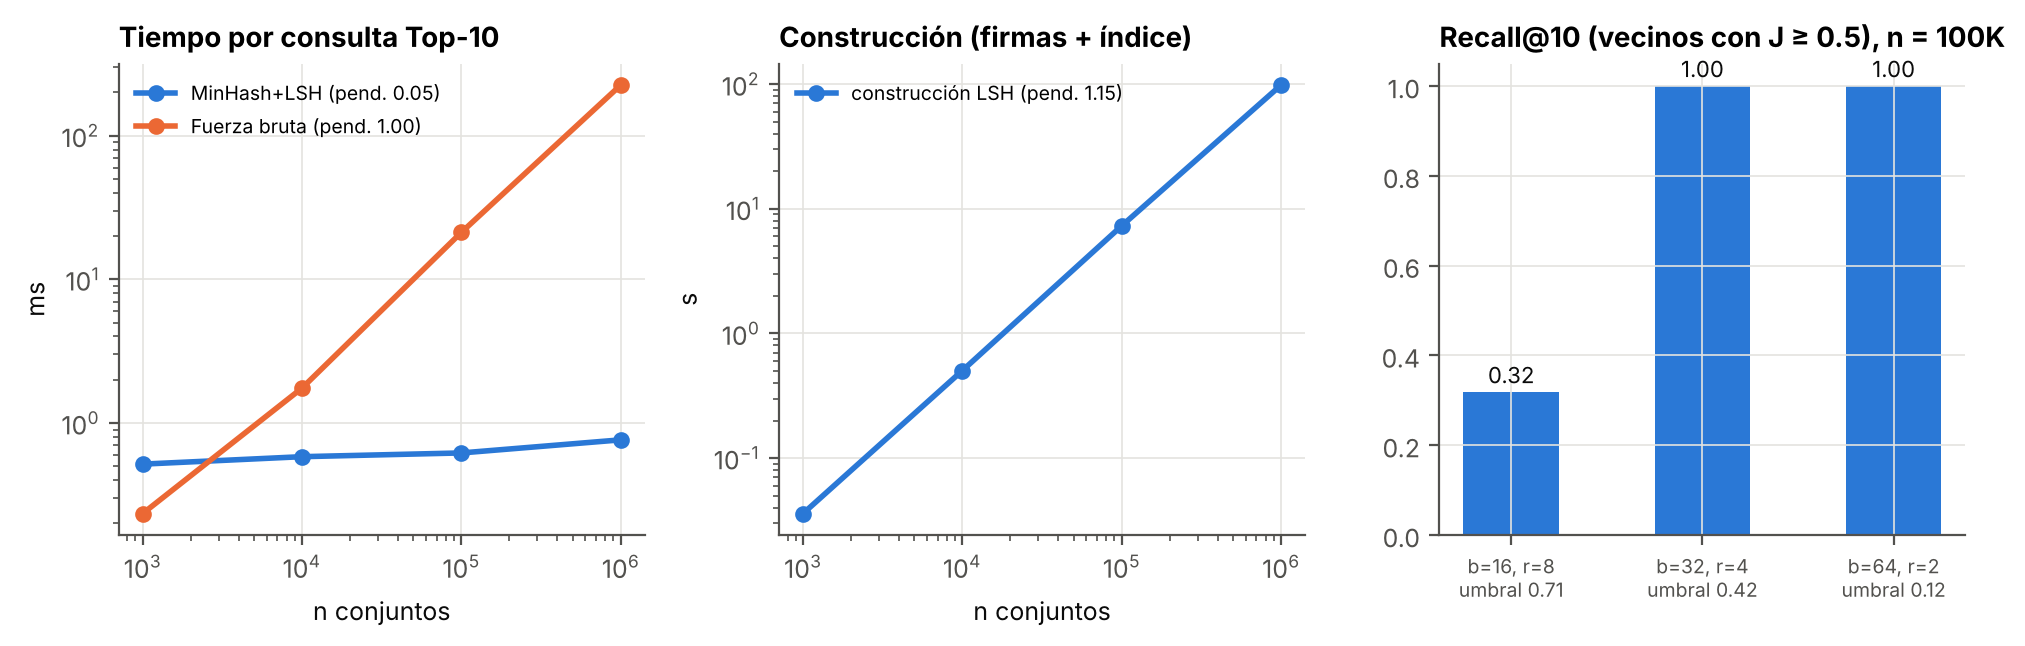
\includegraphics[width=\linewidth]{figures/fig_minhash.png}
  \caption{MinHash + LSH frente a Jaccard exacto por fuerza bruta: tiempo por consulta, construcción y recall según el número de bandas.}
\end{figure}

La consulta LSH se mantiene entre \textbf{0{,}6 y 0{,}8 ms} de 1K a 1M conjuntos (pendiente 0{,}05), mientras la fuerza bruta crece linealmente (pendiente 1{,}00) hasta 225 ms: LSH es \textbf{295 veces} más rápido en 1M, con recall@10 de 1{,}0 sobre los vecinos con $J \ge 0{,}5$. Con 16 bandas (umbral 0{,}71) el recall cae a 0{,}32; con 64 bandas (umbral 0{,}13) se mantiene, pero los candidatos por consulta pasan de 1{,}4 a 3{,}2, lo que confirma la curva en S. El costo está en la construcción (98 s para 1M) y en la memoria de las firmas (1{,}5\,GB = $128 \times 12$\,B $\times$ 1M); por eso se omitió 10M (15\,GB). En el pipeline las firmas se calculan solo para los 200K productos.

\begin{figure}[!htbp]
  \centering
  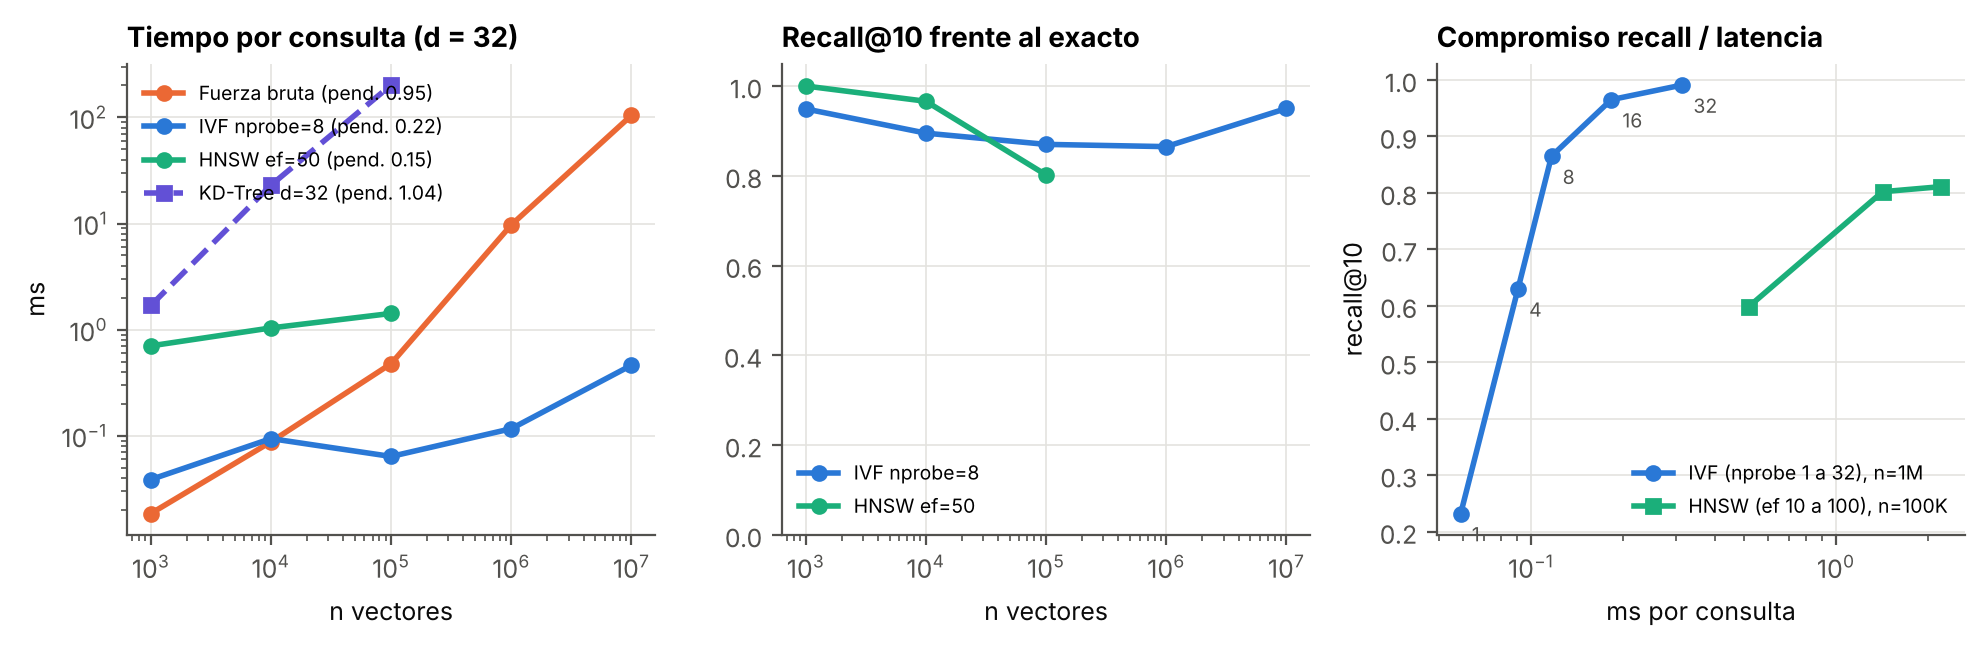
\includegraphics[width=\linewidth]{figures/fig_ann.png}
  \caption{ANN en $d = 32$: IVF y HNSW frente a KNN exacto y al KD-Tree; recall@10 y compromiso recall/latencia.}
\end{figure}

Con 10M vectores de 32 dimensiones, el IVF (4\,096 celdas, $n_\text{probe} = 8$) responde en \textbf{0{,}46 ms frente a 104 ms} del KNN exacto (226 veces) con recall@10 de 0{,}95; con $n_\text{probe} = 16$ sube a 0{,}98 a la mitad de velocidad. En 1M, el barrido de $n_\text{probe}$ de 1 a 32 recorre la curva de recall de 0{,}23 a 0{,}99, que es el parámetro que el sistema ajusta según la latencia permitida. El costo es la construcción (k-means: 145 s en 10M). HNSW en Python puro llegó a recall 0{,}97 en 10K pero a 0{,}80 en 100K con $ef$ de 50 a 100, y su construcción tardó 316 s en 100K, por lo que se limitó a 100K y el pipeline usa IVF. Sin aproximación, el KD-Tree en $d = 32$ fue 420 veces más lento que la fuerza bruta en 100K, porque en alta dimensión casi no poda ramas.

\subsection{Grafo (S8)}

\begin{figure}[!htbp]
  \centering
  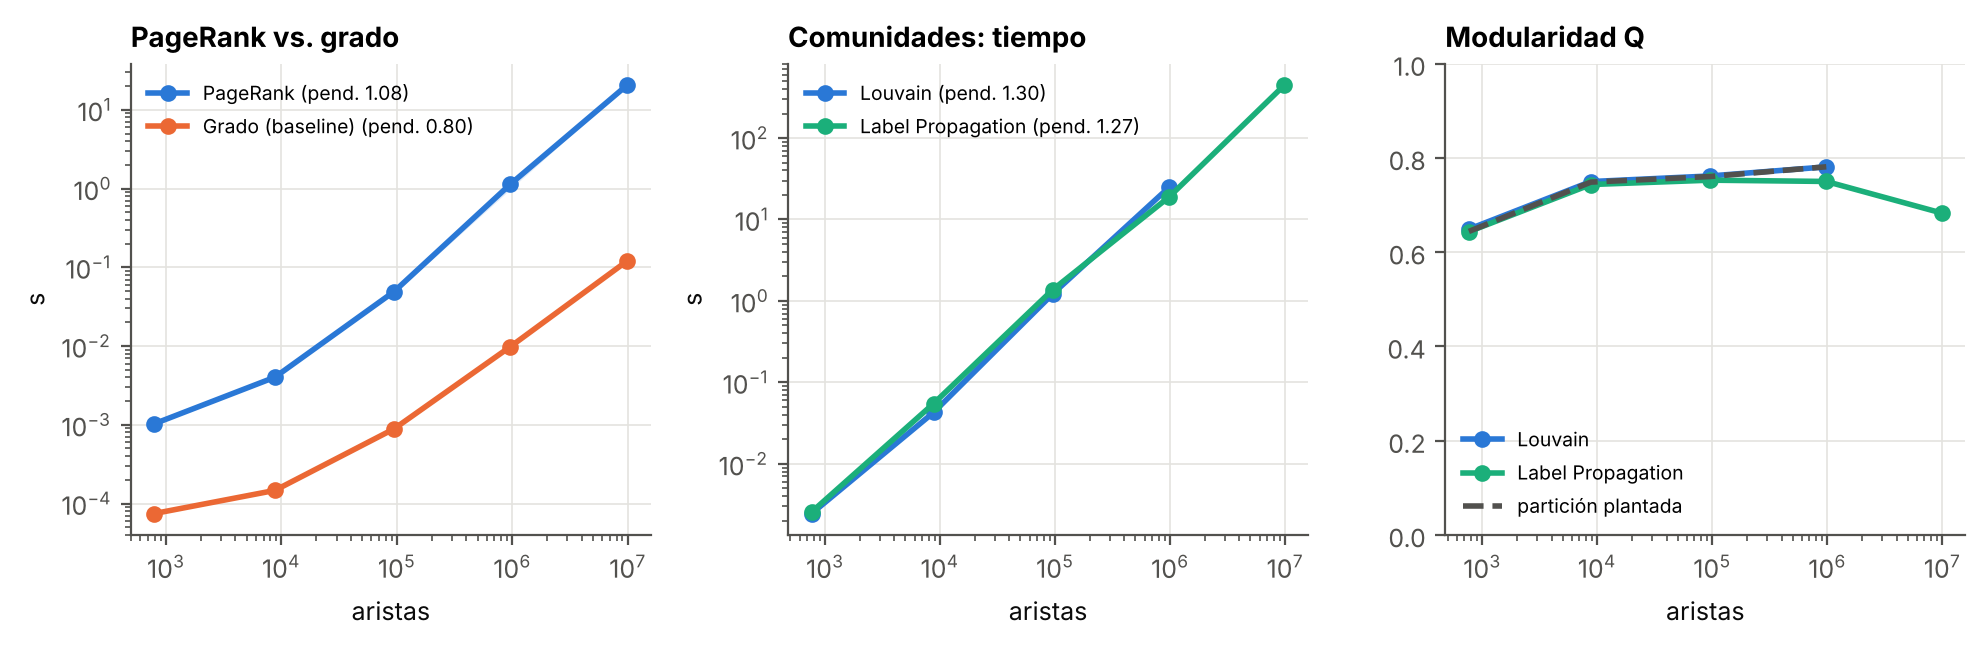
\includegraphics[width=\linewidth]{figures/fig_graph.png}
  \caption{PageRank frente al grado ponderado, y Louvain frente a Label Propagation en grafos con comunidades plantadas.}
\end{figure}

PageRank escala linealmente en aristas (pendiente 1{,}08) y converge en 47 a 56 iteraciones: 20{,}7 s para 9{,}9M aristas. Su correlación de Spearman con el grado ponderado es 0{,}99 y el top-100 coincide en 97\,\%, así que en co-compra la diferencia está en la cola: PageRank sube productos conectados con productos centrales.

En comunidades, sobre grafos con particiones plantadas, Louvain obtiene mayor modularidad que Label Propagation en todos los tamaños (0{,}781 frente a 0{,}750 con 1M aristas, igual a la partición plantada), es más estable entre semillas (NMI 0{,}99 frente a 0{,}94) y recupera mejor la partición real (NMI 0{,}96 frente a 0{,}93), aunque tarda 25 s frente a 19 s. Con 10M aristas solo corrió LPA (448 s), que se fragmentó en 104\,606 comunidades con $Q = 0{,}68$; Louvain en Python puro superó los 40 minutos y se acotó a 1M aristas. En el grafo de co-compra de los datos reales, que es pequeño y disperso porque pocas sesiones compran más de un producto (6\,901 productos y 14\,035 aristas), Louvain logró $Q = 0{,}626$ con 1\,005 comunidades frente a $Q = 0{,}394$ de LPA con 1\,608: la diferencia crece cuando la estructura es débil.

\subsection{Pipeline completo con 10M eventos reales}\label{sec:corrida}

\begin{table}[!htbp]
\centering\small
\begin{tabular}{@{}lr@{\hspace{0.5cm}}lr@{}}
\toprule
\textbf{Etapa} & \textbf{Tiempo (s)} & \textbf{Etapa} & \textbf{Tiempo (s)}\\
\midrule
S0 ingesta (lectura Parquet + cola) & 259 & S4 B+Tree & 3{,}8\\
S1 preprocesamiento & 69 & S5 KD-Tree (consultas + 5 refrescos) & 3{,}0\\
S2 prioridad & 79 & S7 refresco LSH + SVD + IVF (5 veces) & 680\\
S3 almacenamiento e interacciones & 84 & S8 grafo (incremental + 5 refrescos) & 3{,}7\\
S6 filtrado & 50 & S9 servicio & 6{,}7\\
\bottomrule
\end{tabular}
\caption{Tiempo por etapa en la corrida con los 10M eventos reales.}
\end{table}

El total fue de 1\,246 s (8\,204 eventos/s) sobre 10\,223\,169 eventos. Se eliminaron los 151\,081 duplicados inyectados sin falsos positivos, se indexaron 178\,145 órdenes en el B+Tree en disco (altura 3) y la matriz usuario $\times$ producto acumuló 5{,}8M celdas no nulas sobre 1{,}07M usuarios y 120\,565 productos. El refresco de S7 concentra el 55\,\% del tiempo (SVD y k-means sobre la matriz completa); refrescar con menor frecuencia o en paralelo es la mejora más directa. Los productos con mayor PageRank son smartphones Samsung y Apple, los más comprados de la semana. El panel Streamlit (Figura~\ref{fig:panel}) expone la misma traza, las alertas ordenadas por el heap, el Top-K de ventas, el autocompletado con el Trie y las consultas por rango de precio sobre el B+Tree.

\begin{figure}[!htbp]
  \centering
  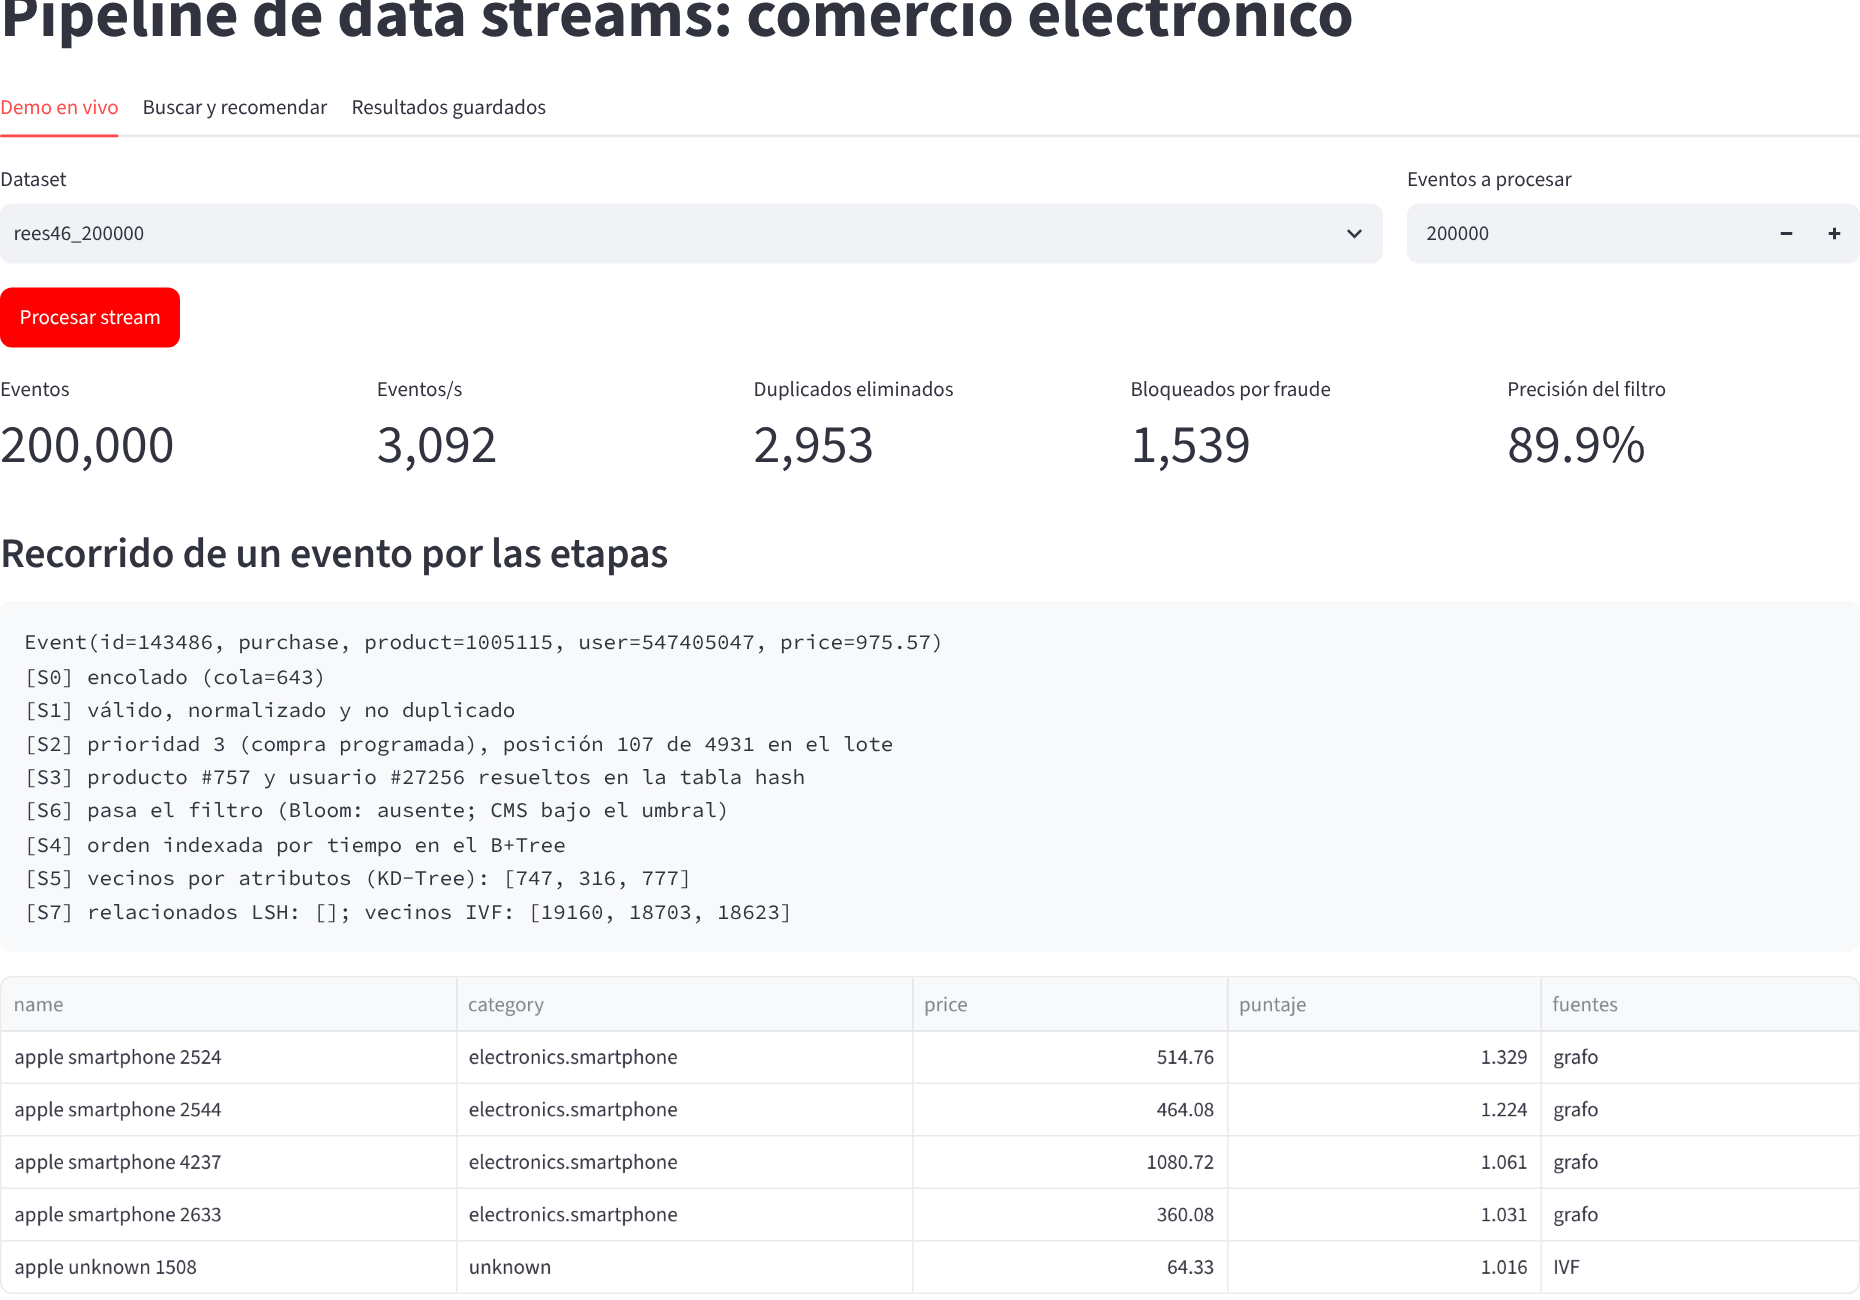
\includegraphics[width=0.6\linewidth]{../docs/capturas/panel_demo.png}
  \caption{Panel de la etapa 9 sobre los primeros 200K eventos reales de REES46.}
  \label{fig:panel}
\end{figure}

% ---------------- 7 ----------------
\section{Conclusiones}

\begin{enumerate}
  \item \textbf{La integración es real y observable.} Un evento atraviesa las 10 etapas y cada salida es la entrada de la siguiente: los índices de S3 son las filas del grafo y de la matriz, la matriz alimenta MinHash y la SVD, y el grafo, el IVF y el KD-Tree se combinan en la recomendación. Una prueba automática lo verifica en cada cambio.
  \item \textbf{Las estructuras aproximadas ganan con error acotado.} Bloom y Count-Min reducen la memoria 22 y 300 veces con errores que coinciden con la teoría; LSH e IVF responden en milisegundos donde la búsqueda exacta es lineal. Donde un error es costoso (bloquear una compra), un paso exacto lo corrige.
  \item \textbf{Las pendientes confirman la complejidad.} Lineal en la cola y la tabla hash, $n\log n$ en ordenación y heap, casi constante en la búsqueda del B+Tree y en el KNN del KD-Tree en baja dimensión, y lineal en todas las líneas base de fuerza bruta.
  \item \textbf{Límites.} Python puro limita las repeticiones en 10M y deja fuera Louvain sobre 10M aristas y MinHash sobre 10M conjuntos; el KD-Tree pierde su ventaja en 32 dimensiones; y en los datos reales el umbral fijo del Count-Min confunde a los usuarios de muy alta frecuencia con fraude.
\end{enumerate}

\subsection{Trabajos futuros}

\begin{itemize}
  \item Procesar octubre y noviembre completos (110M eventos) y calibrar el umbral del Count-Min por usuario.
  \item Paralelizar el refresco de S7, que concentra el 55\,\% del tiempo.
  \item Comparar Leiden con Louvain y usar Counting Bloom para poder retirar tarjetas de la lista negra.
\end{itemize}

% ---------------- Repositorio ----------------
\section*{Repositorio público de GitHub}
\addcontentsline{toc}{section}{Repositorio público de GitHub}

\begin{itemize}
  \item Código, informe, notebook, diagrama, resultados y diapositivas:\\ \url{\repo}
  \item Reproducción:
\begin{Verbatim}[fontsize=\footnotesize]
pip install -r requirements.txt
python -c "import kagglehub; print(kagglehub.dataset_download(\
  'mkechinov/ecommerce-behavior-data-from-multi-category-store'))"
# copiar 2019-Oct.csv a data/raw/
python scripts/prepare_data.py --source rees46 --events 10000000
python scripts/run_pipeline.py --data data/rees46_10000000
python bench/run_benchmarks.py && python bench/plots.py
\end{Verbatim}
\end{itemize}

% ---------------- Referencias ----------------
\section*{Referencias}
\addcontentsline{toc}{section}{Referencias}

{\small
\begin{list}{}{\leftmargin=1.2em\itemindent=-1.2em\itemsep=3pt\parsep=0pt}
\item Bloom, B.~H. (1970). Space/time trade-offs in hash coding with allowable errors. \emph{Communications of the ACM}, 13(7), 422--426. \url{https://doi.org/10.1145/362686.362692}
\item Blondel, V.~D., Guillaume, J.-L., Lambiotte, R. y Lefebvre, E. (2008). Fast unfolding of communities in large networks. \emph{J. Stat. Mech.}, P10008. \url{https://doi.org/10.1088/1742-5468/2008/10/P10008}
\item Brin, S. y Page, L. (1998). The anatomy of a large-scale hypertextual Web search engine. \emph{Computer Networks and ISDN Systems}, 30(1--7), 107--117. \url{https://doi.org/10.1016/S0169-7552(98)00110-X}
\item Broder, A.~Z. (1997). On the resemblance and containment of documents. \emph{Compression and Complexity of Sequences}, 21--29. \url{https://doi.org/10.1109/SEQUEN.1997.666900}
\item Cormen, T.~H., Leiserson, C.~E., Rivest, R.~L. y Stein, C. (2022). \emph{Introduction to Algorithms} (4.ª ed.). MIT Press.
\item Cormode, G. y Muthukrishnan, S. (2005). An improved data stream summary: The Count-Min sketch and its applications. \emph{Journal of Algorithms}, 55(1), 58--75. \url{https://doi.org/10.1016/j.jalgor.2003.12.001}
\item Halko, N., Martinsson, P.~G. y Tropp, J.~A. (2011). Finding structure with randomness: Probabilistic algorithms for constructing approximate matrix decompositions. \emph{SIAM Review}, 53(2), 217--288.
\item Indyk, P. y Motwani, R. (1998). Approximate nearest neighbors: Towards removing the curse of dimensionality. \emph{STOC '98}, 604--613. \url{https://doi.org/10.1145/276698.276876}
\item Jégou, H., Douze, M. y Schmid, C. (2011). Product quantization for nearest neighbor search. \emph{IEEE TPAMI}, 33(1), 117--128. \url{https://doi.org/10.1109/TPAMI.2010.57}
\item Kirsch, A. y Mitzenmacher, M. (2006). Less hashing, same performance: Building a better Bloom filter. \emph{ESA 2006}, 456--467.
\item Leskovec, J., Rajaraman, A. y Ullman, J.~D. (2020). \emph{Mining of Massive Datasets} (3.ª ed.). Cambridge University Press.
\item Malkov, Y.~A. y Yashunin, D.~A. (2020). Efficient and robust approximate nearest neighbor search using hierarchical navigable small world graphs. \emph{IEEE TPAMI}, 42(4), 824--836. \url{https://doi.org/10.1109/TPAMI.2018.2889473}
\item Raghavan, U.~N., Albert, R. y Kumara, S. (2007). Near linear time algorithm to detect community structures in large-scale networks. \emph{Physical Review E}, 76(3), 036106. \url{https://doi.org/10.1103/PhysRevE.76.036106}
\item Samet, H. (2006). \emph{Foundations of Multidimensional and Metric Data Structures}. Morgan Kaufmann.
\item Traag, V.~A., Waltman, L. y van Eck, N.~J. (2019). From Louvain to Leiden: Guaranteeing well-connected communities. \emph{Scientific Reports}, 9, 5233. \url{https://doi.org/10.1038/s41598-019-41695-z}
\end{list}
}

\end{document}
